\documentclass{article}

\usepackage[a-2u]{pdfx}
\usepackage[utf8]{inputenc}
\usepackage[T1]{fontenc}
\usepackage{array}
\usepackage[ddmmyyyy]{datetime}
\usepackage{geometry}
\usepackage{enumitem}
\usepackage{listings}
\usepackage{graphicx}
\graphicspath{{fig/}{wireframe/}}
\usepackage{tabularx}
\usepackage{longtable}
\usepackage{xcolor}
\usepackage{parskip}
\usepackage{nameref}
\usepackage{hyperref}
\usepackage{booktabs}
\usepackage{placeins}

\lstdefinestyle{code}{
  basicstyle=\ttfamily\small,
  breaklines=true,
  frame=single,
  columns=fullflexible,
  keepspaces=true,
  showstringspaces=false,
  keywordstyle=\color{blue},
  commentstyle=\color{gray}
}

\newcommand*{\fullref}[1]{\hyperref[{#1}]{\ref*{#1} \nameref*{#1}}}

\def\twodigits#1{%
    \ifnum#1<10 0\fi
    \number#1}%

\renewcommand{\dateseparator}{.}
\renewcommand{\baselinestretch}{1.5}

\geometry{margin=2cm}

\def\ResearchProject{Research project}
\def\CompanyProject{Company project}
\def\SoftwareProject{Software project}

% METADATA SECTION START
\def\StudentsFullName{Pavol Rajczy}
\def\Obor{Computer Science -- Software and Data Engineering}
\def\ProjetTitle{AI-Assisted Ontology Design and Integration with Dataspecer}
\def\ProjectType{\ResearchProject}
\def\SupervisorFullName{prof. Mgr. Martin Nečaský, Ph.D.}
\def\ConsultantsFullName{Mgr. Štěpán Stenchlák}
% METADATA SECTION END

\title{\ProjetTitle}
\author{\StudentsFullName}

\begin{document}

\centerline{\Large \textbf{Specification of research project}}
\centerline{ \textbf{Department of Software Engineering}}
\centerline{ \textbf{Faculty of Mathematics and Physics, Charles University}}
\bigskip
{\noindent\begin{tabular*}{\textwidth}{ >{\raggedleft}m{4cm} l}
 {\bf Solver:} & \StudentsFullName \\
 {\bf Study program:} & \Obor \\
 & \\
 {\bf Project title:} & \ProjetTitle \\
 {\bf Project type:} & \ProjectType \\
 & \\
 {\bf Supervisor:} & \SupervisorFullName \\
 {\bf Consultants:} & \ConsultantsFullName \\
\end{tabular*}}

\clearpage
\setcounter{tocdepth}{2}
\tableofcontents
\clearpage

\section{Introduction}

In semantic data modeling, \emph{data specifications} describe the structure and meaning of data so that different systems can consistently interpret and validate it. Specifications include vocabularies, application profiles, and derived technical artifacts --- schemas for XML, JSON, CSV, and documentation. Designing such a specification, especially an ontology or vocabulary, is demanding: it requires identifying concepts, relationships, and constraints from expert or legal documents and formalising them.





\subsection{Relation to other projects}
\label{sec:relation}
To support this work, the research group of the project supervisor developed a \textbf{prototype assistant} for \emph{agentic semantic modeling}: it uses large language models (LLMs) to iteratively design an ontology from text --- for example from legislation stored in a \emph{knowledge base}. A knowledge base here means a collection of documents (legal texts, expert literature) from which the assistant proposes classes, attributes, and relationships. The user works in a \emph{design project} where domain areas, iterations, planned tasks per iteration, and---after \emph{prepare}---concrete ontology operations materialised from those tasks are available. Previous development showed that such an assistant is usable, but limitations remain: the assistant's outputs cannot be directly used in the tools the research group and partners use for managing specifications; there is no complete workflow from design through approval and handoff; and there is no systematic user feedback that the assistant would follow.

\textbf{Dataspecer}~\cite{dataspecer} is a tool for managing semantic data specifications: from vocabularies and application profiles to derived technical artifacts --- data schemas, validation rules, APIs, and application prototypes. It allows defining classes, properties, and relationships in RDF Schema style, combining terms from existing vocabularies into application profiles, and semi-automatically deriving schemas for XML, JSON, and CSV --- supporting both semantic and technical data interoperability.
An existing semantic-modeling prototype already demonstrates the basic iterative workflow, but it remains experimental.

The goal of this project is to connect the assistant with Dataspecer and complete the missing workflow: so that the user can \emph{review, edit with feedback (human-in-the-loop), approve, and export the resulting ontology} to Dataspecer --- making the entire process from knowledge base documents to a usable specification in Dataspecer possible without manual transcription. The knowledge base does not have to be tightly bound to the assistant; the document store can be external, and the project only references it.

\section{Project description}

\subsection{Core concepts}

The following terms are used throughout this specification:

\begin{itemize}
  \item \textbf{Ontology} --- a set of classes, attributes, and relationships identified by URIs, representing the domain vocabulary. Classes form a generalisation hierarchy; relationships are directed and connect a source class to a target class.
  \item \textbf{Source ontology} --- the current, authoritative ontology version in a design project. Modified only by explicit operation apply actions or import actions.
  \item \textbf{Knowledge base} --- a collection of domain documents (legal acts, expert texts) belonging to a design project, used by the assistant as source material.
  \item \textbf{Design project} --- the central unit of work: it holds a knowledge base, a source ontology, domain areas, and a list of iterations.
  \item \textbf{Knowledge domain area} --- a thematic section of the domain (e.g. a chapter of a law), identified from the knowledge base, that organises the design work.
  \item \textbf{Design iteration} --- an incremental modeling step planned for a domain area. In \emph{prepare}, the task planner first breaks the iteration into concrete tasks; the modeler then generates ontology edit operations for each task (with task linkage). The user reviews the operations and applies a selected subset.
  \item \textbf{Ontology edit operation} --- an atomic change to an ontology exposed to Dataspecer integration. The currently supported operation types are \texttt{create}, \texttt{update}, and \texttt{remove/delete}; if additional types are needed, they will be agreed with the Dataspecer team.
  \item \textbf{Project guidance item} --- a persistent, typed instruction (instruction, correction, preference, or constraint) that the assistant follows across all calls in a project.
  \item \textbf{Dataspecer exchange format} --- JSON used to import vocabulary snapshots from Dataspecer; export toward Dataspecer uses ontology edit operations, as in \fullref{sec:dataspecer}.
\end{itemize}

\subsection{Context and existing system}

The existing prototype defines the following workflow:

\begin{enumerate}
  \item The user creates a design project and loads domain documents into it.
  \item The assistant analyses the documents and proposes thematic domain areas.
  \item The user selects a domain area and asks the assistant to suggest modeling iterations for it.
  \item The user selects an iteration and triggers preparation: the assistant plans concrete tasks and generates ontology edit operations for each task.
  \item The user applies the operations; the ontology grows incrementally.
  \item The process repeats across areas and iterations until the ontology is complete.
\end{enumerate}

The following gaps prevent the prototype from being used in real workflows:

\begin{itemize}
  \item Operation semantics are not yet aligned as an explicit integration contract with Dataspecer; operation handling remains prototype-level.
  \item There is no structured preview of proposed changes before apply.
  \item There is no mechanism to approve or reject individual operations.
  \item User feedback (corrections, preferences) is not recorded or fed back to the assistant in any systematic way.
  \item The only frontend is a debug application unsuitable for production use.
\end{itemize}



\subsection{User groups}

The system is designed to satisfy the following user groups:

\begin{itemize}
  \item \textbf{Ontology designer}, who uses the assistant to build a new vocabulary or extend an existing one from domain documents. They may be a domain expert (e.g. a legal expert or a data architect) rather than a programmer.
  \item \textbf{Dataspecer user}, who already works in Dataspecer and wants to use the assistant without leaving the Dataspecer environment.
  \item \textbf{Advanced user}, who is an expert ontology engineer and wants to use the assistant in a targeted way: selecting specific parts of the ontology, specifying goals, and managing detailed guidance.
  \item \textbf{Assistant developer}, who needs the system to be maintainable, extensible, testable, and well-documented.
\end{itemize}

\subsection{User stories}
\label{sec:user-stories}

User stories for \textit{Ontology designer}:
\begin{enumerate}[label=\textbf{US-\protect\twodigits{\arabic*}:},align=left,leftmargin=1.4cm]
  \item As an ontology designer, I want to create a design project with a target ontology URI and load domain documents into it, so that I have a clear context for my design work.
  \item As an ontology designer, I want the assistant to analyse the knowledge base and propose domain areas, so that I can organise the ontology design work into manageable thematic sections.
  \item As an ontology designer, I want the assistant to suggest modeling iterations for a selected domain area, so that I have a plan for incrementally extending the ontology.
  \item As an ontology designer, I want the task planner to decompose a planned iteration into concrete tasks against the current ontology, so that I can see a clear work breakdown before any ontology changes are generated.
  \item As an ontology designer, I want to prepare a planned task so that the modeler produces ontology edit operations, which I can review before apply, so that I understand exactly what will change in the ontology and how that maps to each task and to the iteration.
  \item As an ontology designer, I want to selectively approve or reject individual operations before applying them, so that I maintain precise control over the ontology content.
  \item As an ontology designer, I want to apply only explicitly approved operations to the source ontology, so that every ontology change is intentional and reviewable.
  \item As an ontology designer, I want to view the current state of the source ontology and operation history at any point, so that I can monitor the overall progress.
  \item As an ontology designer, I want to export the current source ontology to a format importable in Dataspecer, so that the designed vocabulary becomes available for data specification work.
\end{enumerate}

User stories for \textit{Dataspecer user}:
\begin{enumerate}[resume,label=\textbf{US-\protect\twodigits{\arabic*}:},align=left,leftmargin=1.4cm]
  \item As a Dataspecer user, I want to import an existing Dataspecer specification as the source ontology for a design project, so that I can extend an already published vocabulary.
  \item As a Dataspecer user, I want to work with the assistant and Dataspecer side by side in two windows, so that I can see the current state of the Dataspecer specification while driving the assistant.
  \item As a Dataspecer user, I want to export the designed ontology back to Dataspecer with a single action after my approval, so that the result is immediately available as a Dataspecer vocabulary.
\end{enumerate}

User stories for \textit{Advanced user}:
\begin{enumerate}[resume,label=\textbf{US-\protect\twodigits{\arabic*}:},align=left,leftmargin=1.4cm]
  \item As an advanced user, I want to define a subarea of the ontology (a subset of classes and relationships) that the assistant should focus on, so that iterations and operations do not stray into parts I consider complete.
  \item As an advanced user, I want to specify a textual goal for the assistant (e.g. ``add attributes for section 3 of the act''), so that the assistant plans iterations toward my stated objective rather than proposing generic iterations.
  \item As an advanced user, I want to manage persistent project guidance items (add, edit, delete instructions, corrections, preferences, and constraints), so that the assistant consistently respects my preferences across all calls.
  \item As an advanced user, I want to save the reason for rejecting an operation as a correction guidance item with a single action, so that the assistant avoids the same mistake in future suggestions.
  \item As an advanced user, I want to view a history of past iterations, decisions, and guidance items, so that I can understand how the ontology evolved and trace the rationale for design choices.
\end{enumerate}

User stories for \textit{Assistant developer}:
\begin{enumerate}[resume,label=\textbf{US-\protect\twodigits{\arabic*}:},align=left,leftmargin=1.4cm]
  \item As an assistant developer, I want to add a new LLM provider by implementing a well-defined abstract interface, so that the system is not tied to OpenAI.
  \item As an assistant developer, I want automated tests for core business logic, so that I can refactor and extend the system with confidence.
\end{enumerate}

\section{Use cases}
\label{sec:use-cases}

This section describes representative end-to-end scenarios.

\subsection{UC-01\quad New ontology from a domain document}
\label{sec:uc-01}

\begin{description}[leftmargin=3.8cm,style=nextline]
  \item[Actors] Ontology designer
  \item[Based on user stories] US-01, US-02, US-03, US-04, US-05, US-06, US-07, US-08, US-09, US-11, US-16
  \item[Goal] Build a new domain vocabulary from uploaded documents using the AI assistant.
  \item[Pre-conditions]
    \begin{itemize}
      \item The user has access to the assistant and is working in a Dataspecer project context.
      \item At least one domain document is available locally.
    \end{itemize}
  \item[Trigger] In Dataspecer, the user clicks the control that opens the assistant; the assistant opens for that project.
\end{description}

\paragraph*{Basic flow.}
\begin{enumerate}
  \item The assistant opens from Dataspecer; the user uploads a domain document and a new design project is created (or attached); the source ontology starts empty. The document is ingested and processed.
  \item Domain area analysis runs after the document has been processed; the assistant proposes thematic areas corresponding to the main sections of the document.
  \item The user selects the first domain area and requests iteration suggestions.
  \item The user selects the first iteration; the task planner decomposes the iteration into concrete tasks against the current source ontology.
  \item For each planned task, the modeler generates linked ontology edit operations.
  \item The user reviews the operation preview: the projected additions match expectations; one proposed class is misnamed. The user rejects that operation, saves the rejection reason as a correction guidance item, and applies the remaining operations.
  \item The user repeats this cycle (task planning, operation generation, review, apply) for subsequent iterations and areas until the vocabulary is complete. Each time the user confirms and applies operations, the updated source ontology is synchronized to Dataspecer automatically.
\end{enumerate}

\paragraph*{Alternative flows.}
\begin{itemize}
  \item[7a.] Synchronization with Dataspecer fails when applying operations. The user retries after correcting connectivity or other issue.
\end{itemize}

\paragraph*{Post-conditions.}
\begin{itemize}
  \item An updated ontology exists in the design project.
  \item Applied changes are reflected in Dataspecer through the automatic sync on apply.
\end{itemize}

\subsection{UC-02\quad Extending an existing Dataspecer specification}
\label{sec:uc-02}

\begin{description}[leftmargin=3.8cm,style=nextline]
  \item[Actors] Ontology designer; Dataspecer user
  \item[Based on user stories] US-03, US-04, US-05, US-06, US-07, US-08, US-09, US-10, US-11, US-12
  \item[Goal] Extend an existing Dataspecer vocabulary with a new domain area without losing the existing content.
  \item[Pre-conditions]
    \begin{itemize}
      \item A vocabulary already exists in Dataspecer and has a publicly accessible specification URL.
      \item The user can open the assistant alongside Dataspecer.
    \end{itemize}
  \item[Trigger] In Dataspecer, the user clicks the control that opens the assistant; the assistant opens for that project.
\end{description}

\paragraph*{Basic flow.}
\begin{enumerate}
  \item The user opens the assistant from Dataspecer; populating the source ontology with the existing content.
  \item In the assistant, the user uploads a document covering the new domain area; after ingestion and processing, domain area analysis runs for that material.
  \item The user plans and prepares iterations; for each iteration, the task planner creates concrete tasks and the modeler generates operations.
  \item The user reviews operations, and applies selected operations. Each confirmed apply synchronizes the updated source ontology to Dataspecer automatically.
  \item The user optionally repeats iteration cycles until the new domain area is adequately covered; Dataspecer stays aligned through the same apply-triggered synchronization.
\end{enumerate}

\paragraph*{Alternative flows.}
\begin{itemize}
  \item[3a.] The assistant proposes a class that already exists. The user rejects the operation and saves a guidance item instructing the assistant to check for duplicates.
  \item[4a.] Synchronization with Dataspecer fails when applying operations. The user retries after correcting connectivity or other issue.
\end{itemize}

\paragraph*{Post-conditions.}
\begin{itemize}
  \item The existing ontology content is preserved (aside from intentional additions applied by the user).
  \item Applied changes are reflected in Dataspecer through the automatic sync on apply.
\end{itemize}

\subsection{UC-03\quad Goal-directed subarea design}
\label{sec:uc-03}

\begin{description}[leftmargin=3.8cm,style=nextline]
  \item[Actors] Ontology designer; Advanced user
  \item[Based on user stories] US-04, US-05, US-07, US-13, US-14
  \item[Goal] Focus the assistant exclusively on a specific subset of the ontology to fill a targeted gap.
  \item[Pre-conditions]
    A design project with an existing source ontology exists.
  \item[Trigger] The user identifies a gap in the vocabulary and defines a subarea to address it.
\end{description}

\paragraph*{Basic flow.}
\begin{enumerate}
  \item The user selects a subarea by choosing the relevant classes.
  \item The user opens the iteration suggester, provides the goal (e.g. \textit{``Add data attributes for section 12 of the act to the existing classes in this subarea''}, and requests iterations.
  \item The assistant proposes iterations scoped to the subarea. The user prepares the first iteration: the task planner fills the task list, then the modeler generates operations per task; the user reviews the resulting operations.
  \item All operations are within the specified subarea; the user applies a selected subset (or all) of them. Confirmed apply actions synchronize the updated ontology to Dataspecer.
\end{enumerate}

\paragraph*{Alternative flows.}
\begin{itemize}
  \item[3a.] The assistant proposes an operation outside the subarea. The user rejects it and adds a constraint guidance item to reinforce the subarea boundary.
\end{itemize}

\paragraph*{Post-conditions.}
\begin{itemize}
  \item The identified gap in the subarea has been addressed.
  \item Changes accepted via apply are reflected in Dataspecer through the automatic sync on apply.
\end{itemize}

\subsection{UC-04\quad HITL correction feedback loop}
\label{sec:uc-04}

\begin{description}[leftmargin=3.8cm,style=nextline]
  \item[Actors] Ontology designer; Advanced user
  \item[Based on user stories] US-06, US-16, US-17
  \item[Goal] Correct a recurring naming issue in the assistant's output and persist the correction for future iterations.
  \item[Pre-conditions]
    A design project with an active task is in progress.
  \item[Trigger] The assistant generates an operation that violates a project naming convention.
\end{description}

\paragraph*{Basic flow.}
\begin{enumerate}
  \item The user rejects the incorrectly named operation.
  \item The user saves the rejection reason (e.g. \textit{``Relationships to legal entities must use the prefix `has', not `is\_connected\_to' ''}) as a correction guidance item.
  \item The user drops unapplied operations introduced by the current iteration.
  \item The user triggers prepare again; the assistant incorporates the correction in its prompt and produces correctly named operations.
\end{enumerate}

\paragraph*{Alternative flows.}
\begin{itemize}
  \item[4a.] The assistant still produces an incorrect name. The user refines the wording of the guidance item and triggers prepare once more.
\end{itemize}

\paragraph*{Post-conditions.}
\begin{itemize}
  \item The correction guidance item is persisted and applied to all subsequent agent calls in the project.
  \item The operations produced after the correction follow the naming convention.
  \item When the user applies the revised operations, the source ontology update is propagated to Dataspecer through the same apply-triggered synchronization as in UC-01--UC-03.
\end{itemize}

\subsection{Wireframes (illustrative)}
\label{sec:wireframes}

The figures below are low-fidelity wireframes of the intended assistant user interface. They illustrate the workflows described in the use cases above and are \emph{not} binding visual design; the implementation may differ while preserving the same functional structure.

\begin{figure}[!htbp]
  \centering
  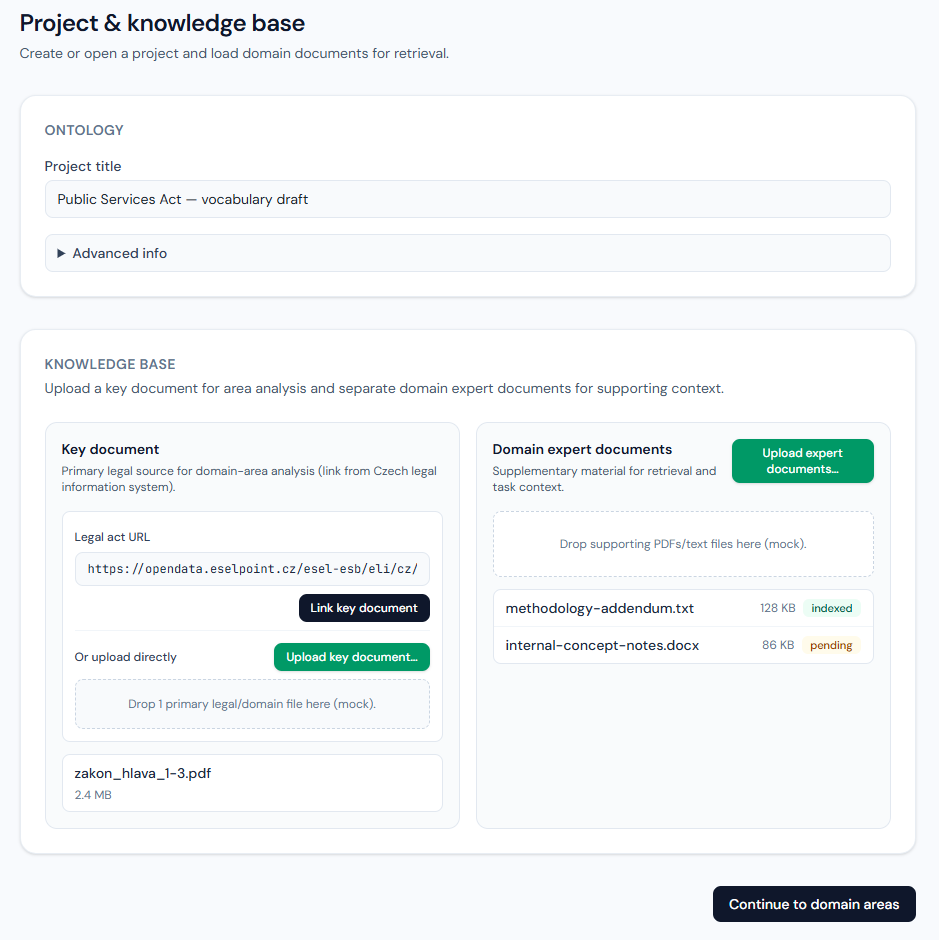
\includegraphics[width=\linewidth,height=0.34\textheight,keepaspectratio]{kb.png}
  \caption{Wireframe: project and knowledge base setup.}
  \label{fig:wf-kb}
\end{figure}

\begin{figure}[!htbp]
  \centering
  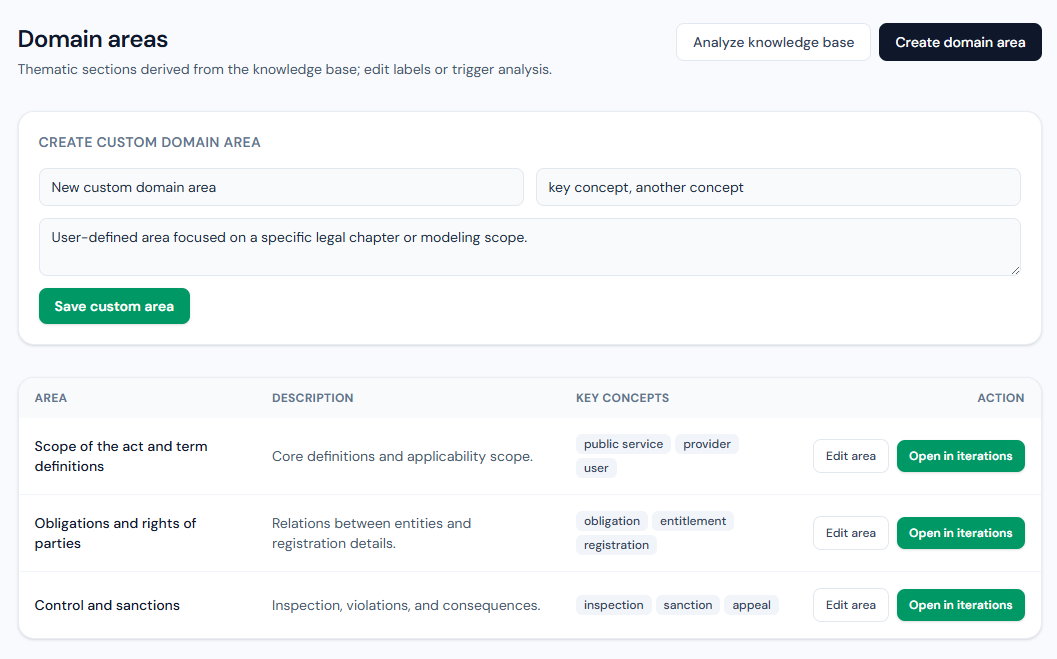
\includegraphics[width=\linewidth,height=0.34\textheight,keepaspectratio]{domarea.png}
  \caption{Wireframe: domain areas.}
  \label{fig:wf-domarea}
\end{figure}

\begin{figure}[!htbp]
  \centering
  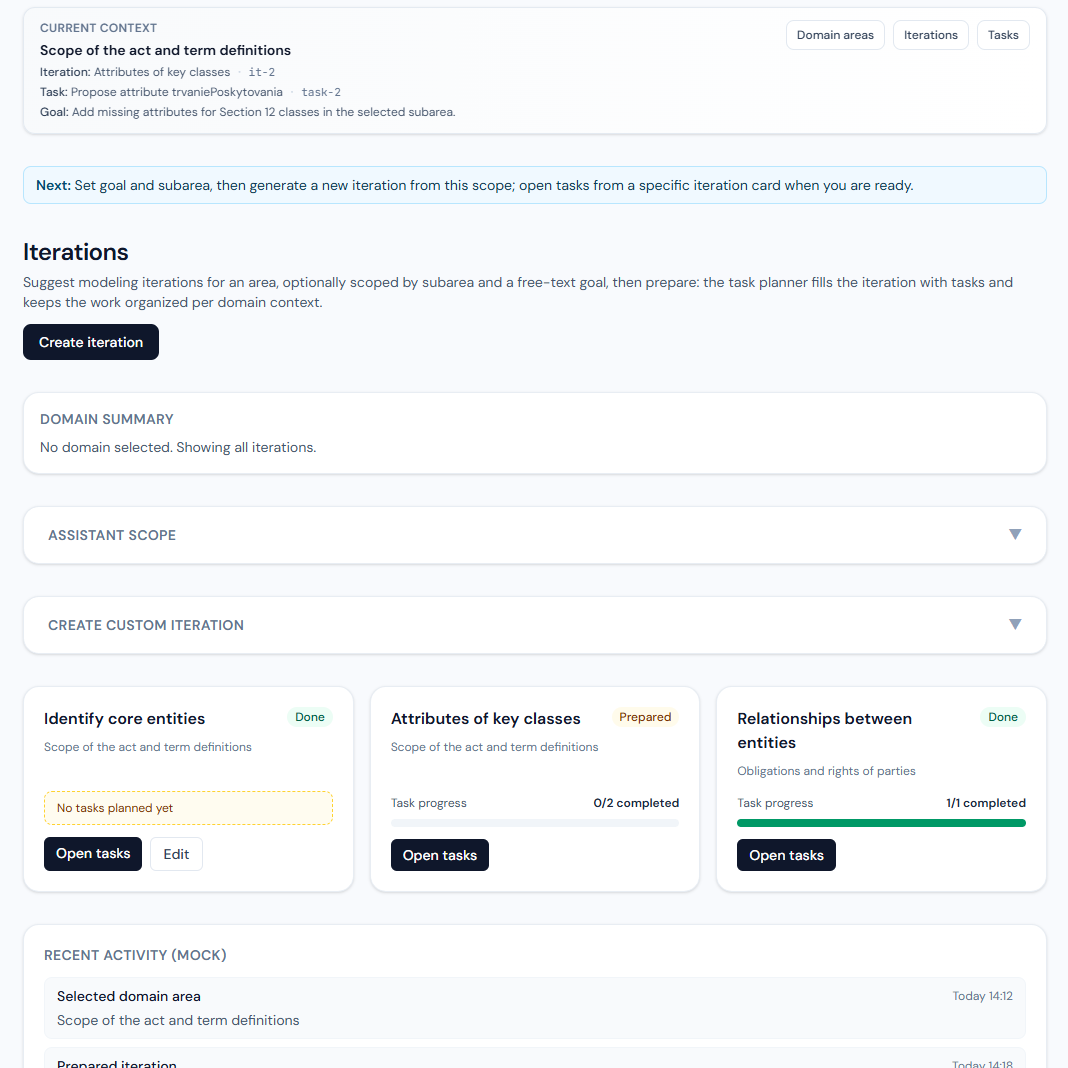
\includegraphics[width=\linewidth,height=0.34\textheight,keepaspectratio]{iter.png}
  \caption{Wireframe: design iterations.}
  \label{fig:wf-iter}
\end{figure}

\begin{figure}[!htbp]
  \centering
  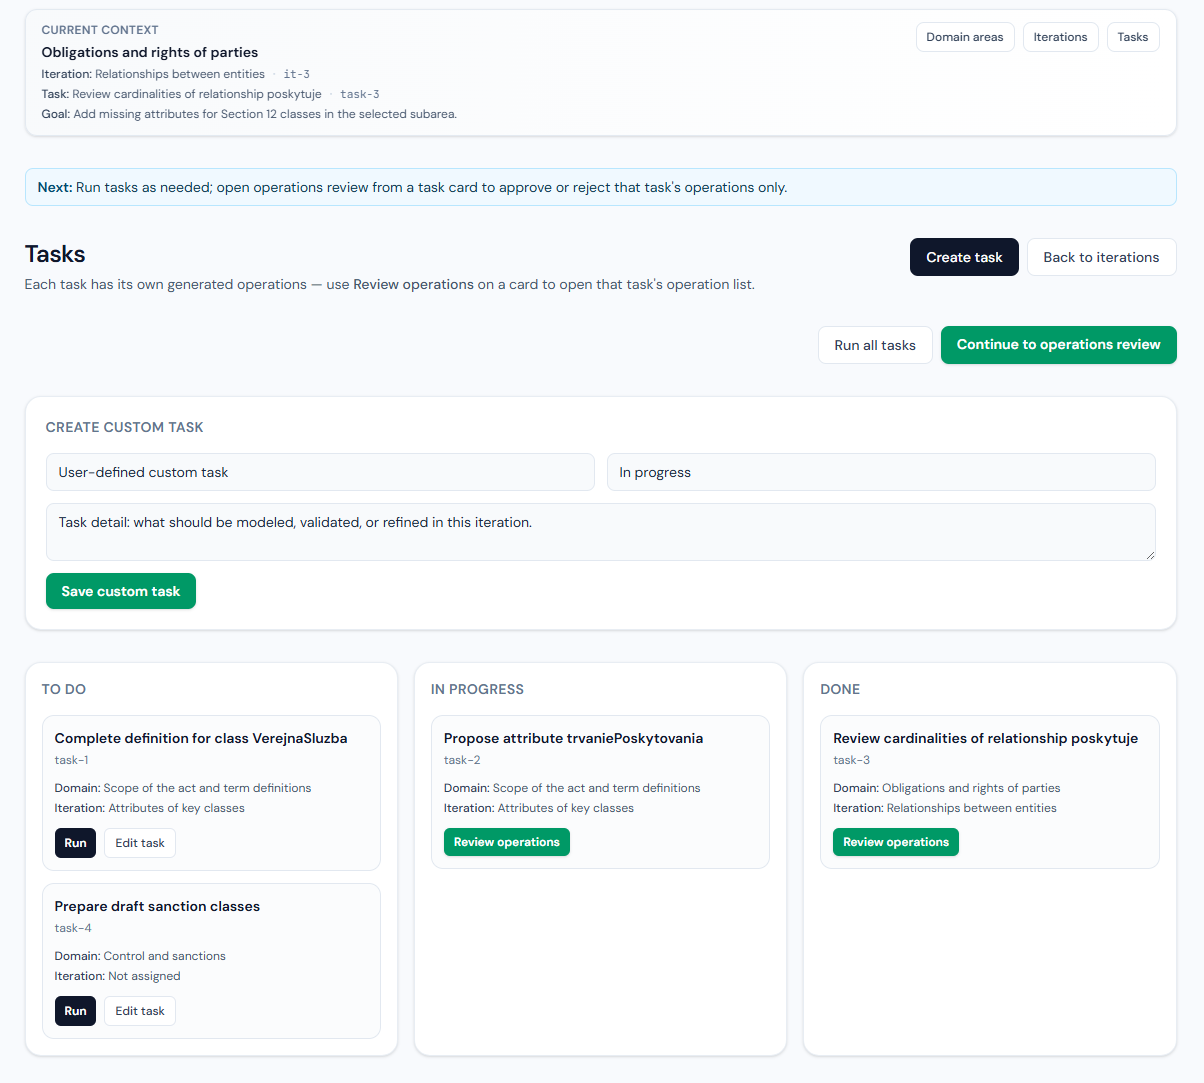
\includegraphics[width=\linewidth,height=0.34\textheight,keepaspectratio]{task.png}
  \caption{Wireframe: planned tasks for an iteration.}
  \label{fig:wf-task}
\end{figure}

\begin{figure}[!htbp]
  \centering
  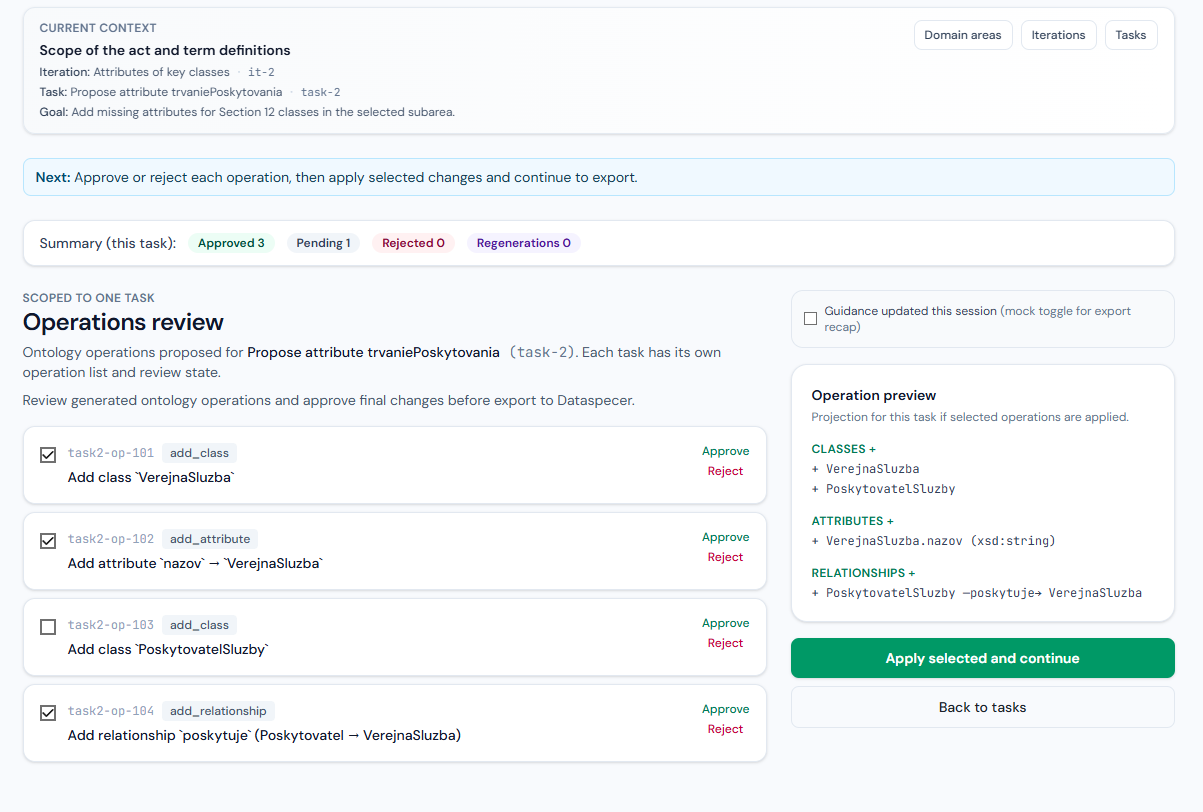
\includegraphics[width=\linewidth,height=0.34\textheight,keepaspectratio]{oper.png}
  \caption{Wireframe: ontology operations review (preview / approve--reject).}
  \label{fig:wf-oper}
\end{figure}

\begin{figure}[!htbp]
  \centering
  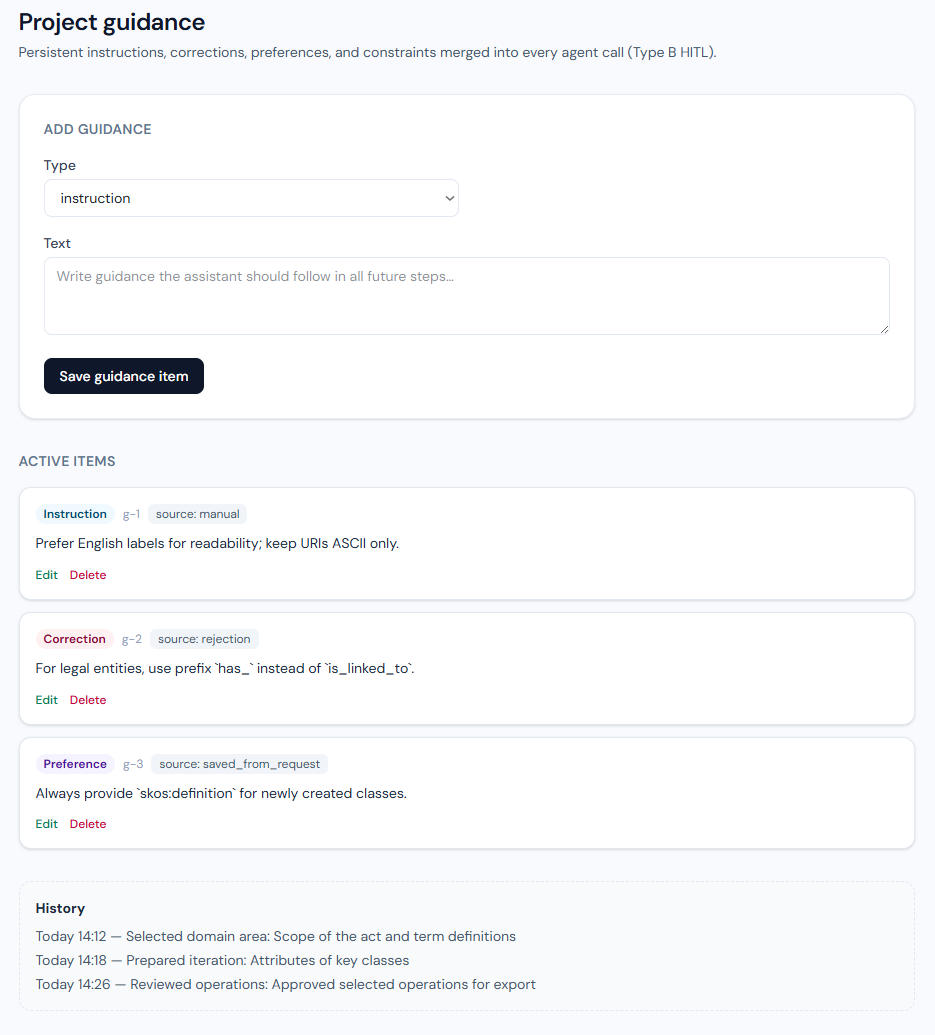
\includegraphics[width=\linewidth,height=0.34\textheight,keepaspectratio]{guid.png}
  \caption{Wireframe: project guidance (instructions / corrections).}
  \label{fig:wf-guid}
\end{figure}

\FloatBarrier
\subsection{Non-Functional requirements}

\subsubsection*{Maintainability}
\begin{enumerate}[label=\textbf{NFR-\protect\twodigits{\arabic*}:},align=left,leftmargin=1.5cm]
  \item The backend shall follow a consistent layered architecture: controllers call services, services use domain objects, stores handle persistence.
  \item Each agent shall implement an abstract base class so that alternative implementations (e.g. different LLM providers) can be substituted without changing service code.
  \item The codebase shall include automated unit tests for service-layer business logic and integration tests for key API scenarios.
\end{enumerate}

\subsubsection*{Extensibility}
\begin{enumerate}[resume,label=\textbf{NFR-\protect\twodigits{\arabic*}:},align=left,leftmargin=1.5cm]
  \item Adding a new LLM provider shall require only implementing the abstract agent interfaces and registering the new implementation in the dependency wiring.
  \item Adding a new operation type shall require only implementing the operation handler and registering it; no changes to the orchestration flow shall be necessary.
\end{enumerate}

\subsubsection*{Security}
\begin{enumerate}[resume,label=\textbf{NFR-\protect\twodigits{\arabic*}:},align=left,leftmargin=1.5cm]
  \item API keys and credentials shall be managed via environment variables; no secrets shall appear in source code or committed data files..
\end{enumerate}

\subsubsection*{Usability}
\begin{enumerate}[resume,label=\textbf{NFR-\protect\twodigits{\arabic*}:},align=left,leftmargin=1.5cm]
  \item The diff and preview displays shall be sufficiently clear that a domain expert without programming knowledge can identify all proposed additions, modifications, and removals within 5 minutes of viewing, without requiring any explanation from a developer.
  \item The frontend shall not require the user to manually manipulate JSON; all interactions shall be through the graphical interface.
  \item The frontend shall provide clear feedback for long-running LLM operations (loading indicators, and where supported, streaming output).
\end{enumerate}

\subsubsection*{Architectural and delivery constraints}
\begin{enumerate}[resume,label=\textbf{NFR-\protect\twodigits{\arabic*}:},align=left,leftmargin=1.5cm]
  \item The production frontend shall be a standalone React application running alongside Dataspecer in a separate browser window for side-by-side work.
\item \textbf{Inbound synchronization (Dataspecer~$\rightarrow$~assistant).} The assistant may continuously refresh its view of the source ontology accordingly, so that vocabulary changes performed manually in Dataspecer are detected without requiring any user action in the assistant.
  \item \textbf{Outbound synchronization (assistant~$\rightarrow$~Dataspecer).} The assistant shall never write to Dataspecer silently. Every outbound change shall be triggered by an explicit user action in the assistant.  
  \item The Dataspecer exchange format shall be the primary stable integration contract. LLM traffic shall go through the LLM gateway. Dataspecer HTTP and payload mapping shall be isolated in the Dataspecer gateway and invoked only from \textbf{design project orchestration}; ontology management shall not call Dataspecer or depend on its API---it receives ontology state and persistence instructions from orchestration only.
\end{enumerate}

\section{Architecture}

The assistant is organised around a \textbf{design project}: it references domain documents in project storage, maintains ontology state in a single authoritative \emph{source} ontology (with explicit apply for changes), and drives \textbf{structured interaction} through the API---domain-area analysis, iteration planning, task preparation, and review of proposed operations---rather than a single open-ended chat session. Optional per-request instructions and persistent \textbf{project guidance} are merged into prompts sent to language models. Retrieval over chunked documents (RAG) supplies task-relevant text to modeling steps via embeddings stored in a per-project index.

\subsection{Architecture views (C4)}

Following the C4 model~\cite{c4model}, the diagrams below use three of its views: \textbf{Level~1 (system context)}---the system in its environment; \textbf{Level~2 (containers)}---major deployable parts and persistence; \textbf{Level~3 (components)}---logical building blocks inside the \textbf{Assistant backend} container. The code-level view is omitted here. Figures~\ref{fig:arch-SystemContext}--\ref{fig:arch-Component} match the workspace model; narrative subsections elaborate behaviour without repeating every edge label.

\begin{figure}[!htbp]
  \centering
  \includegraphics[width=\linewidth,height=0.64\textheight,keepaspectratio]{SystemContext-001.png}
  \caption{C4 Level~1: system context (actors and external systems relevant to the assistant).}
  \label{fig:arch-SystemContext}
\end{figure}

\begin{figure}[!htbp]
  \centering
  \includegraphics[width=\linewidth,height=0.64\textheight,keepaspectratio]{Container-001.png}
  \caption{C4 Level~2: containers (e.g.\ user-facing app, API service, persistence).}
  \label{fig:arch-Container}
\end{figure}

\begin{figure}[!htbp]
  \centering
  \includegraphics[width=\linewidth,height=0.64\textheight,keepaspectratio]{Component-001.png}
  \caption{C4 Level~3: components inside the backend (e.g.\ knowledge services, agent orchestration, project state).}
  \label{fig:arch-Component}
\end{figure}

\clearpage

\subsection{System overview}

At Level~1 (Figure~\ref{fig:arch-SystemContext}), the assistant depends on two external software systems: \textbf{Dataspecer}, for specification management and vocabulary import/export, and an \textbf{LLM provider}, for embeddings and agent-side calls. Other actors and relationships are as shown in the figure.

At Level~2 (Figure~\ref{fig:arch-Container}), the assistant is split into \textbf{five} containers: \textbf{assistant frontend} (React/Vite SPA), \textbf{assistant backend} (Python/FastAPI), \textbf{vector database} (FAISS index for embeddings and chunk metadata), \textbf{knowledge base files storage} (raw and preprocessed KB documents), and \textbf{project and ontology storage} (projects, source ontology and related state, operation history, guidance). The frontend communicates with the backend over REST/JSON. How these containers map to processes or folders in deployment is left open; the diagram states the logical separation.

\paragraph{Backend components (C4 Level~3).}
Figure~\ref{fig:arch-Component} sketches the inside of the assistant backend: REST API, design project orchestration, knowledge base service, ontology management, agent pipeline, guidance, LLM gateway, and Dataspecer gateway. Relationships (including which parts talk to FAISS vs.\ file stores) follow the diagram; this document does not nail down every method signature or future refactor.

\paragraph{Typical control flow.}
End-to-end behaviour (prepare, review, apply, export) is described in the use cases and later subsections. Outbound LLM and Dataspecer traffic is intended to go through the dedicated gateways rather than ad hoc calls scattered across the codebase. User-triggered sync toward Dataspecer remains as in the non-functional requirements.

\subsection{Knowledge base and retrieval}
\label{sec:kb-retrieval}

Documents are loaded from URLs or files provided by the user. The knowledge base service reads and writes \textbf{knowledge base files storage} and builds or updates the \textbf{vector database} container; the agent pipeline consumes retrieved chunks from that index for RAG. Ontology and guidance persistence use \textbf{project and ontology storage} as in Figure~\ref{fig:arch-Container}.

\subsection{Design project ontology state}
\label{sec:ontology-state}

The \textbf{ontology management} component (Figure~\ref{fig:arch-Component}) maintains the project's ontology state (including apply and history as modeled). It does not fetch specifications from Dataspecer: when import is requested, \textbf{design project orchestration} retrieves and validates the exchange-format payload via the Dataspecer gateway and supplies ontology management with the deserialized state to persist. Conceptually the design project still binds identity, knowledge-base references, domain areas, iterations, and the ontology snapshot updated through apply or import. Preview and diff behaviour is described below and may be refined in implementation.

After project creation or ontology import, the source ontology is the baseline for subsequent work. The user runs iterations (prepare, then apply selected operations), and every successful apply updates the source ontology immediately. Iteration records, applied operations, and guidance history remain persisted to preserve traceability of design decisions.

\subsection{Agent pipeline}
\label{sec:agent-pipeline}

The agent pipeline consists of four abstract roles, each with a default LLM-backed implementation: a \emph{domain-area analyzer} (proposes thematic areas from the key document), an \emph{iteration suggester} (proposes design iterations for an area, optionally constrained by a user subarea and goal), a \emph{task planner} (breaks an iteration into concrete tasks against the current source ontology), and a \emph{modeler} (produces ontology edit operations for each task from retrieved passages and the current ontology). All roles receive the merged project guidance and any one-off user instruction.

The \emph{prepare} step for a planned iteration loads the project, merges guidance with the request-specific instruction, asks the task planner to fill the iteration's task list from the current source ontology, then for each task retrieves relevant knowledge-base snippets and invokes the modeler. Each generated operation is stored with identity and linkage to its task; nothing is applied to the source ontology yet. The iteration is marked as having generated operations and the project is saved.

After prepare, the operations are available for inspection and selective approval; they are not applied to the source ontology until the user explicitly invokes \emph{apply}.

\subsubsection{Subarea and goal injection}

When the user provides a subarea (a list of class URIs), it is passed to the iteration suggester and encoded as an additional constraint in the prompt---effectively restricting proposals and operations to those classes and their immediate neighbourhood. The modeler receives the same constraint.

When the user provides a goal (a free-text statement), it is passed to the iteration suggester as an explicit planning objective, replacing the default open-ended prompt. This enables targeted modeling sessions without changing the overall workflow structure.

\subsection{Preview, diff, and operation-level HITL}
\label{sec:hitl-a}

\subsubsection{Preview (projected diff)}

After prepare, the user can request a \emph{preview}: a structured projection of the source ontology state after a given set of operations is applied, computed without modifying the stored source ontology. The response groups projected additions, modifications, and removals, each partitioned into classes, attributes, and relationships with the usual identifiers and human-readable labels where applicable.

\subsubsection{Selective apply}

The apply action accepts an optional subset of operation identifiers. Only those operations are applied to the source ontology; the rest remain on the iteration as still-planned and can be applied later or dropped. If no subset is given, all pending operations from the prepare step are applied.

\subsubsection{Rejection and correction}

When the user rejects an operation, they may supply a rejection reason. The system can persist that reason as a correction-type guidance item so later agent calls avoid repeating the same mistake.

\subsection{Dataspecer integration}
\label{sec:dataspecer}

The \emph{Dataspecer exchange format} defines JSON payloads for bringing vocabulary state \emph{from} Dataspecer into the assistant. Architecturally, all Dataspecer-facing HTTP and JSON/schema mapping live in the \textbf{Dataspecer gateway}, which \textbf{design project orchestration} calls when a workflow step requires import or export (Figure~\ref{fig:arch-Component}). The \textbf{ontology management} component does not reference Dataspecer URLs or schemas; orchestration delivers the validated snapshot (or receives edit operations for export) and drives persistence through the ontology component.

\paragraph{Import (JSON).}
Inbound integration uses \textbf{JSON} in the Dataspecer exchange format: orchestration retrieves the document from a given URL (or equivalent source) via the gateway, validates against the published schema, deserializes into the internal ontology representation, and instructs ontology management to persist. The snapshot enters the assistant as structured JSON, not as a sequence of edit operations.

\paragraph{Export (ontology edit operations toward Dataspecer).}
Outbound integration pushes changes toward Dataspecer as \textbf{ontology edit operations} that Dataspecer exposes or accepts on its side. The vocabulary of operation types follows Dataspecer; for now it comprises \texttt{create}, \texttt{update}, and \texttt{remove/delete}. Further kinds may be added as the Dataspecer-side contract evolves, in coordination with the Dataspecer team. Sending when the user confirms apply or uses export controls follows the same user-initiated sync rules as elsewhere in this specification.

\subsection{Frontend}

The production frontend is a standalone React single-page application that runs in a separate browser window alongside Dataspecer. The user works with both windows open side by side: Dataspecer shows the specification state, and the assistant window drives the design workflow. The stack aligns with the container diagram (Figure~\ref{fig:arch-Container}): TypeScript, React, Vite, TanStack Router, TanStack Query, and Tailwind CSS.

\paragraph{Linear workflow stepper.}
Between domain analysis and export, the mock shows a horizontal \emph{workflow stepper} with five steps: \textbf{Domain areas} $\rightarrow$ \textbf{Iterations} $\rightarrow$ \textbf{Tasks} $\rightarrow$ \textbf{Operations} $\rightarrow$ \textbf{Export}. Steps after the first are linked with workflow context (\texttt{domainId}, \texttt{iterationId}, \texttt{taskId}) carried in URL search parameters so that iterations, tasks, and operations views stay scoped to the same domain area and iteration. Project setup and guidance sit outside this chain but remain always reachable from the sidebar.

\paragraph{Screen-level responsibilities.}
\begin{enumerate}
  \item \textbf{Project \& knowledge base} (\texttt{/project}) --- project title, target ontology URI, key document URL or upload, supplementary expert documents; entry point for aligning the project with Dataspecer import when implemented.
  \item \textbf{Domain areas} (\texttt{/domain-areas}) --- list and edit domain areas; trigger domain-area analysis.
  \item \textbf{Iterations} (\texttt{/iterations}) --- list iterations for the selected domain; optional \textbf{goal} text and \textbf{subarea} (class URIs); suggest iterations; prepare a planned iteration (task list then operations).
  \item \textbf{Tasks} (\texttt{/tasks}) --- Kanban-style task board for the iteration; link into operations review per task.
  \item \textbf{Operations review} (\texttt{/operations}) --- operations for the selected task; preview diff panel; approve, reject (with optional reason for guidance), or regenerate proposals; banner toward apply/export when ready.
  \item \textbf{Guidance} (\texttt{/guidance}) --- manage persistent guidance items (instructions, corrections, preferences, constraints).
  \item \textbf{Export result} (\texttt{/export-result}) --- recap after apply/export (counts of approved, pending, rejected operations; optional guidance-updated flag; link back to operations), consistent with explicit user-triggered sync toward Dataspecer.
\end{enumerate}

Structured preview and diff are emphasised on the \textbf{operations review} screen; a dedicated full-ontology browser may be added in implementation but is not required for the mock baseline. Import/export affordances in the UI should remain consistent with orchestration-driven use of the Dataspecer gateway described above.


\section{Technologies}

\paragraph{Backend.}
Python 3.11+, FastAPI, Uvicorn, OpenAI Python client (GPT-4o and embedding models), rdflib (OWL/Turtle loading and export), sentence-transformers / FAISS (semantic indexing), docling (legal document parsing), spaCy, httpx, pytest.

\paragraph{Frontend.}
TypeScript, React 18, Vite, TanStack Router, TanStack Query, Tailwind CSS.

\section{Evaluation}
\label{sec:evaluation}

The project will be evaluated through a user study with approximately 5 participants, focused on the usability of the implemented solution. Each participant will be given a domain document and, where applicable, an existing Dataspecer specification to extend, and asked to use the assistant to design an ontology from these inputs and export the result back to Dataspecer.

The evaluation scenario will cover the main use cases described in Section~\ref{sec:use-cases}. During the study it will be observed whether the participants can run domain-area analysis, prepare a design iteration, review the generated tasks and ontology edit operations, approve or reject operations (including saving a rejection as a correction guidance item), apply the approved operations, and export the resulting ontology to Dataspecer. The focus is on whether the main concepts of the assistant are understandable and whether the overall workflow can be completed with reasonable effort.

Usability will be assessed using the System Usability Scale (SUS) questionnaire completed after the task. As a supporting evaluation layer, the project also includes automated tests: unit tests for service-layer logic (operation apply, diff computation, guidance injection) and API-level integration tests for key endpoints.

\section{Risks}

\begin{longtable}{| p{5cm} | p{5cm} | p{5cm} |}
\hline
\textbf{Risk} & \textbf{Likelihood / Impact} & \textbf{Mitigation} \\
\hline
LLM output quality is insufficient for the target domain (e.g. low-quality operations requiring too many rejections). & Medium / High & Prompt engineering with guidance items and RAG retrieval; the HITL correction loop is designed to iteratively improve quality. The system works regardless of LLM quality; it only affects the number of rejection cycles. \\
\hline
Dataspecer Dataspecer exchange format or API changes incompatibly during the project. & Low / Medium & Use only the published, versioned JSON schema (\texttt{v1.0}); validate every import and export against it. API integration is optional; export/import via file/URL is the primary path. \\
\hline
Knowledge base FAISS index grows too large for fast in-process retrieval. & Low / Medium & Chunk-level retrieval with a configurable top-$k$ limit. The longer-term solution depends on how KB storage evolves (see \fullref{sec:kb-retrieval}). \\
\hline
Frontend integration into Dataspecer is blocked by internal Dataspecer changes. & Medium / Medium & The frontend communicates with the backend via a stable REST API; it can be deployed as a standalone app that deep-links with Dataspecer until native integration is complete. \\
\hline
Concurrent edits from external tools may desynchronise the ontology state used by the assistant. & Low / Low & The source ontology is modified through apply and import endpoints in this system; external updates are synchronised through explicit re-import from Dataspecer before further assistant iterations. \\
\hline
\end{longtable}

\section{Milestones / Deliverables}

A live demonstration is expected to be presented to the commission. The milestone table below uses relative months from the project start.

\begin{longtable}{|l|p{10cm}|l|}
\hline
 & \textbf{Milestone} & \textbf{Target} \\
\hline
\endfirsthead
\hline
 & \textbf{Milestone} & \textbf{Target} \\
\hline
\endhead
\textbf{M1} & Source ontology state workflow implemented; operation apply endpoint; operation history persistence & Month 1 \\
\hline
\textbf{M2} & Diff and preview endpoints implemented; structured diff response format & Month 2 \\
\hline
\textbf{M3} & Operation-level HITL: selective apply, rejection endpoint, save-as-guidance from rejection & Month 3 \\
\hline
\textbf{M4} & Subarea and goal parameters added to IterationSuggester and Modeler agents; tested end-to-end & Month 4 \\
\hline
\textbf{M5} & Dataspecer import/export fully integrated into project workflow; Dataspecer format schema validation & Month 4 \\
\hline
\textbf{M6} & Frontend MVP: project management, iterations, operations review, diff view; runs alongside Dataspecer & Month 5 \\
\hline
\textbf{M7} & Frontend complete: guidance management, history view, subarea selector, export UI & Month 6 \\
\hline
\textbf{M8} & Testing, polishing, user study with approx.\ 5 participants and SUS questionnaire, documentation & Month 6 \\
\hline
\textbf{M9} & Live demonstration to the commission; incorporate feedback from demo & Month 7 \\
\hline
\textbf{M10} & Project submission & Month 7 \\
\hline
\end{longtable}

\clearpage
\section{Time Schedule}

\hskip-0.5cm
\begin{longtable}{ | m{13em} | m{18em} | m{2.5cm} | m{1.3cm} | }
   \hline
 Milestone / Deliverable & Activity & Schedule & Man-days \\
 \hline
 M1: Source ontology state & Design source ontology state model; implement apply-based update flow and operation history persistence & Month 1 & 10 \\
 \hline
 M2: Diff and preview & Implement diff and preview endpoints; structured diff response format & Month 2 & 8 \\
 \hline
 M3: HITL & Operation-level approve/reject API; save-as-guidance from rejection & Month 3 & 8 \\
                 & API integration tests & Month 3 & 4 \\
 \hline
 M4: Subarea + goal & Extend iteration suggester and modeler agents; add parameters to API & Month 4 & 8 \\
                    & Testing & Month 4 & 3 \\
 \hline
 M5: Dataspecer workflow & Finalise Dataspecer format export/import integration; schema validation; workflow tests & Month 4 & 6 \\
 \hline
 M6: Frontend MVP & React components for project, KB, iterations, operations review, diff view; Dataspecer integration & Month 5 & 20 \\
 \hline
 M7: Frontend complete & Guidance management UI; subarea selector; export/import UI; history view & Month 6 & 15 \\
 \hline
 M8: Testing + docs & Prepare evaluation scenario covering the main use cases; recruit approx.\ 5 participants & Month 6 & 3 \\
                    & Run user study sessions and collect SUS questionnaire responses & Month 6 & 5 \\
                    & Analyse SUS results and observations; fix identified issues; write project documentation & Month 6 & 6 \\
 \hline
 M9: Demonstration & Prepare and deliver live demonstration to the commission; address review comments & Month 7 & 4 \\
 \hline
 M10: Submission & Final submission package & Month 7 & 2 \\
 \hline
\end{longtable}

\section{Form of collaboration}

\subsection{Consulting plan}

The research group meets weekly; in addition, the student meets with the supervisor every two weeks to review design decisions, completed milestones, and any blockers. For quick day-to-day communication the group uses Mattermost.
Beyond meetings, collaboration may include asynchronous technical review---for example feedback from the supervisor or consultant on pull requests in the project's Git repository and comparable code-review workflows.

\subsection{Collaboration with other team members}

Coordination with the Dataspecer team is needed to keep the assistant aligned with the two integration contracts owned by Dataspecer (detailed in \fullref{sec:dataspecer}) and to agree on any future deeper integration between the two tools.

\begin{thebibliography}{9}
\bibitem{c4model}
S. Brown. \textit{The C4 model for visualising software architecture}. Available at \url{https://c4model.com/}.
\bibitem{dataspecer}
Dataspecer project. \textit{Dataspecer: Tool for Data Specification Management}. Available at \url{https://dataspecer.com}.
\end{thebibliography}

\end{document}
